\documentclass[11pt]{article}

\usepackage{amsmath}
\usepackage{tikz}
\usepackage{pgfplots}
\usepackage{subcaption}
\usepackage[left=0.5cm,right=0.5cm,top=0.5cm,bottom=0.5cm]{geometry}

\begin{document}
	\begin{figure}[t]
		\begin{subfigure}[t]{0.32\textwidth}
			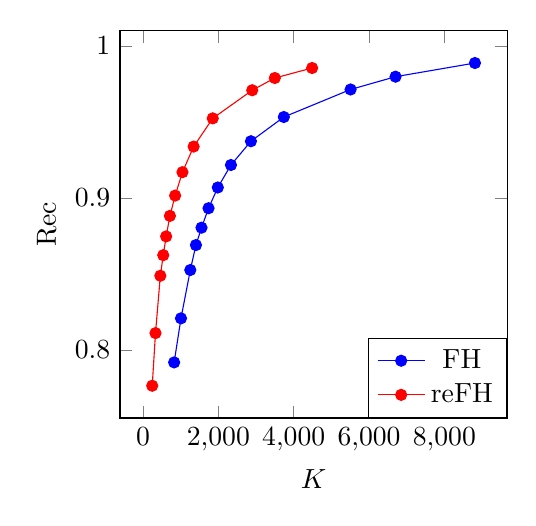
\begin{tikzpicture}
				\begin{axis}[
					legend style={
						at={(1,0)},
						anchor=south east
					},
					xlabel=$K$,
					ylabel=$\text{Rec}$,
					yticklabel style={
        					/pgf/number format/fixed,
        					/pgf/number format/precision=5
					},
					height=6.5cm,
					width=6.5cm]
						\addplot[blue,mark=*] coordinates{
							(826.888, 0.791822)
							(1008.37, 0.820798)
							(1256.1, 0.852576)
							(1405.27, 0.868974)
							(1553.3, 0.880399)
							(1739.63, 0.893199)
							(1985.52, 0.906827)
							(2334.99, 0.921621)
							(2864.92, 0.937254)
							(3738.44, 0.953177)
							(5510.46, 0.97129)
							(6703.26, 0.979699)
							(8811.13, 0.988687)
						};
						\addlegendentry{FH}
						
						\addplot[red,mark=*] coordinates{
							(244.941, 0.776467)
							(331.829, 0.811089)
							(460.512, 0.848784)
							(537.439, 0.862329)
							(614.644, 0.874673)
							(714.639, 0.88816)
							(853.039, 0.901519)
							(1047.45, 0.916895)
							(1344.25, 0.93373)
							(1851.18, 0.952298)
							(2899.2, 0.970778)
							(3499.02, 0.978829)
							(4489.13, 0.985405)
						};
					\addlegendentry{reFH}
				\end{axis}
			\end{tikzpicture}
		\end{subfigure}
		\begin{subfigure}[t]{0.32\textwidth}
			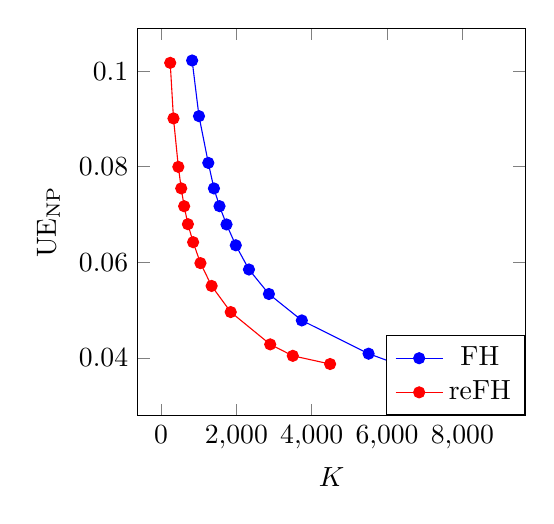
\begin{tikzpicture}
				\begin{axis}[
					legend style={
						at={(1,0)},
						anchor=south east
					},
					xlabel=$K$,
					ylabel=$\text{UE}_{\text{NP}}$,
					yticklabel style={
        					/pgf/number format/fixed,
        					/pgf/number format/precision=5
					},
					height=6.5cm,
					width=6.5cm]
						\addplot[blue,mark=*] coordinates{
							(826.888, 0.102232)
							(1008.37, 0.0905894)
							(1256.1, 0.0808087)
							(1405.27, 0.0754681)
							(1553.3, 0.0717517)
							(1739.63, 0.0679285)
							(1985.52, 0.0635661)
							(2334.99, 0.0585009)
							(2864.92, 0.0533748)
							(3738.44, 0.0478442)
							(5510.46, 0.0408878)
							(6703.26, 0.0374582)
							(8811.13, 0.0347051)
						};
						\addlegendentry{FH}
						
						\addplot[red,mark=*] coordinates{
							(244.941, 0.10174)
							(331.829, 0.0901138)
							(460.512, 0.0799742)
							(537.439, 0.0754728)
							(614.644, 0.0717433)
							(714.639, 0.0679849)
							(853.039, 0.0642173)
							(1047.45, 0.0598369)
							(1344.25, 0.0550612)
							(1851.18, 0.0495942)
							(2899.2, 0.0428342)
							(3499.02, 0.040439)
							(4489.13, 0.0387244)
						};
					\addlegendentry{reFH}
				\end{axis}
			\end{tikzpicture}
		\end{subfigure}
		\begin{subfigure}[t]{0.32\textwidth}
			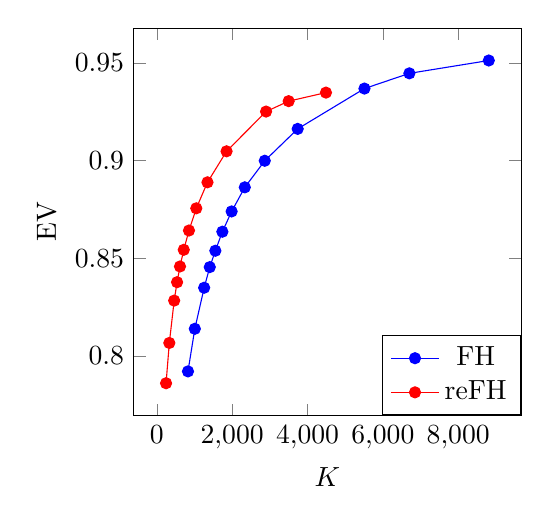
\begin{tikzpicture}
				\begin{axis}[
					legend style={
						at={(1,0)},
						anchor=south east
					},
					xlabel=$K$,
					ylabel=$\text{EV}$,
					yticklabel style={
        					/pgf/number format/fixed,
        					/pgf/number format/precision=5
					},
					height=6.5cm,
					width=6.5cm]
						\addplot[blue,mark=*] coordinates{
							(826.888, 0.792009)
							(1008.37, 0.813817)
							(1256.1, 0.834838)
							(1405.27, 0.845403)
							(1553.3, 0.853786)
							(1739.63, 0.863524)
							(1985.52, 0.873913)
							(2334.99, 0.886249)
							(2864.92, 0.899864)
							(3738.44, 0.916183)
							(5510.46, 0.936821)
							(6703.26, 0.94462)
							(8811.13, 0.951196)
						};
						\addlegendentry{FH}
						
						\addplot[red,mark=*] coordinates{
							(244.941, 0.785951)
							(331.829, 0.806575)
							(460.512, 0.828261)
							(537.439, 0.837688)
							(614.644, 0.845735)
							(714.639, 0.854266)
							(853.039, 0.864139)
							(1047.45, 0.875514)
							(1344.25, 0.888828)
							(1851.18, 0.904706)
							(2899.2, 0.925049)
							(3499.02, 0.930381)
							(4489.13, 0.934755)
						};
					\addlegendentry{reFH}
				\end{axis}
			\end{tikzpicture}
		\end{subfigure}
	\end{figure}
\end{document}